%%
%% Template intro.tex
%%

\chapter{Mapping the Night Sky}
\label{cha:astro}
When many people think about astronomy, the first things that pop into their mind are
breathtaking images of the sky like the famous Hubble Deep Field. But pretty images alone
are not enough to do real science. For us to make any meaningful observations about
astronomical objects, we need actual quantitative measurements.

\section{Spectroscopy and Photometry}
\label{sec:spec}

One such quantitative approach is spectroscopy. This involves
using diffraction grating to disperse light and measure the amount of electromagnetic radiation,
or flux, emitted from an object at small wavelength intervals. As the name implies, we end
up with a spectrum, like the one shown in Figure \ref{fig:vega}. The shape of the spectrum
and its absorption lines allow us to deduce many useful properties such as the object's
temperature and chemical composition.

Unfortunately, it can be very costly to take high resolution spectra of faint objects since
we are spreading light thinly across many wavelengths. Photometry gets around this problem
by separating light into fewer groups and thus reducing the wavelength resolution
\cite{romanishin02}. Specifically we have a set of filters, each of which can be put in
front of the CCD
camera to allow only light from certain wavelengths to pass through. Associated with
each filter is a transmission function $T(\lambda)$ that tells us
the fraction of light that the filter will transmit at wavelength $\lambda$.
Figure \ref{fig:vega} shows $T(\lambda)$ of the five bandpasses (u, g, r, i, and z) that
are used in the SDSS.

\begin{figure}[tbp]
	\centering
	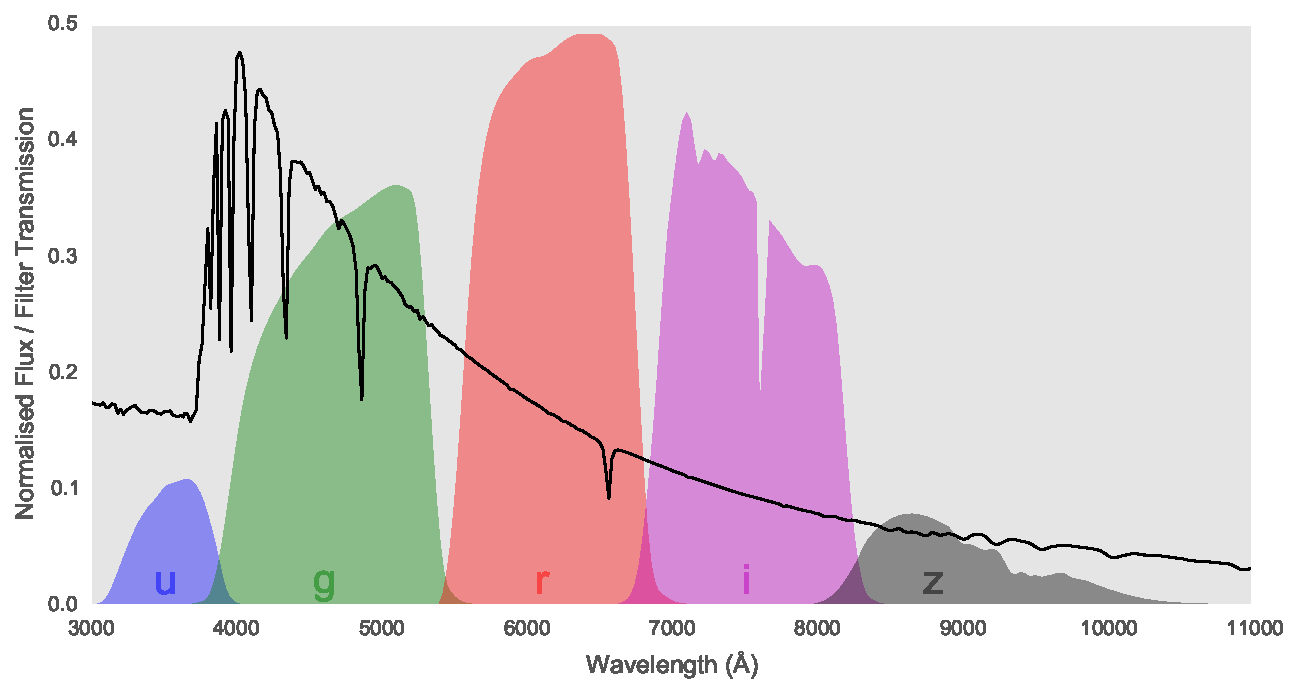
\includegraphics[width=\textwidth]{figures/vega_filters_and_spectrum}
	\caption[The spectrum of the star Vega and the ugriz bandpasses]{The black curve
		is the spectrum of Vega, the fifth brightest star in the night sky. The spectrum
		tells us how much radiation Vega emmits at each wavelength. We also show five
		transmission functions, one for each of the five ugriz filters. The transmission
		function tells us how much light can get through the filter at each wavelength.}
	\label{fig:vega} \index{Vega}
\end{figure}


\section{Measuring Fluxes and Magnitudes}
\label{sec:mag}
When light hits the CCD, all we have initially are counts of photons, one for each pixel.
The first challenge is to assign the photons to distinct objects. Two models are used
in the SDSS, depending on whether we assume the object is an extended source or a point source.


\subsection{Petrosian Flux}
Galaxies are extended-source objects so we need to define an aperture radius, within which
all the photons are added together to obtain the flux of the galaxy. Since galaxies have
poorly defined edges, a consistent method to pick the aperture radius is required.
\shortciteN{blanton01} define a quantity called the Petrosian ratio:
	\begin{IEEEeqnarray*}{lCl}
		\mathfrak{R}_p(r) = \frac{\int_{0.8r}^{1.25r} 2\pi s I(s) \, ds}{\pi (1.25^2 - 0.8^2) r^2}
							\bigg/ \frac{\int_0^r 2\pi s I(s) \, ds}{\pi r^2}
	\end{IEEEeqnarray*}
This is the ratio of the mean local surface brightness over an annulus at $r$ to the mean
surface brightness within $r$. The quantity $I(r)$ is the galaxy surface brightness profile
and can be estimated from the photon count. With this, we define the Petrosian
radius $r_p$ as the radius such that $\mathfrak{R}_p(r_p) = 0.2$. This is one of the features
in the SDSS dataset that will prove to be very useful in distinguishing galaxies from
point-source objects. The aperture radius is then chosen to be $2r_p$ to ensure that almost
all of the light from a typical galaxy is captured. Finally for each bandpass, we can calculate
the corresponding Petrosian flux as
	\begin{IEEEeqnarray*}{lCl}
		f &=& \int_{0}^{2 r_p} 2 \pi s I(s) \, ds
	\end{IEEEeqnarray*}

\subsection{Point Spread Function Fitting}
Stars, quasars, and white dwarfs are unresolved point sources so they can be modelled by a point
spread function (PSF). This approach is particularly useful when we examine a dense region
like a globular cluster. In such places, given the amount of overlap, it would be very
difficult define an aperture that includes only photons from an object and excludes all others
from the neighbours. In PSF fitting, we assume that all objects have the same shape, which allows
us to fit a Gaussian model to each of them. We then iteratively vary the position and flux
of the objects until the model produces the observed light distribution \cite[Chapter 10]{palmer01}.
The flux estimated by the converged model is called the PSF flux.


\subsection{Magnitudes}
The fluxes of the brightest and the dimmest objects in the sky can differ by many orders of
magnitudes. This motivates us to take one step further and convert fluxes to inverse
hyperbolic sine (or arsinh) magnitudes:
	\begin{IEEEeqnarray*}{lCl}
		m &=& -\frac{2.5}{\ln(10)} \Bigg[ \arsinh\bigg(\frac{f/f_0}{2b}\bigg) + \ln(b) \Bigg]
	\end{IEEEeqnarray*}
Here $f_0$ is the flux of the object with a conventional magnitude of 0 and $b$ is the
softening parameter. A nice feature of this magnitude system is that for bright objects
with a high signal-to-noise ratio, it behaves like a logarithmic scale, i.e. with
every decrease of 1 in the magnitude scale, the object becomes 2.5 times brighter.\footnote{
	The reader might wonder why the scale works in reverse, with a small magnitude
	corresponding to more brightness. This is the convention created two centuries ago by
	the Greek astronomer Hipparchus, which, for better or worse, has stuck with us ever since.}
At the same time, as the flux tends toward zero for fainter objects, the arsinh function
(unlike the log function) ensures that the magnitudes are still well-defined \cite{lupton99}.


\section{Equatorial Coordinate System}
Imagine a very large celestial sphere with Earth at its centre. By projecting onto the
inside surface of this sphere, we have a way to specify the position
of any astronomical object. In this thesis, we will mainly use the equatorial coordinate system,
where an object's position is specified by two numbers, a right ascension (ra) and a declination
(dec).

The origin of this coordinate system is defined as follows. Anything on the celestial sphere that is
directly above the Earth's equator will have a declination of 0\deg. To define a zero point
for the right ascension, we use the fact that the centre of the Sun passes through the plane of the
Earth's equator twice a year. The first crossing point usually happens on 21 March and is called
the vernal equinox. We now define the right ascension of the vernal equinox to be
0\deg~\cite[Chapter~1]{sparke07}.\footnote{
	There is actually a slight complication. Since the Earth's rotation axis is not
	fixed due to precession, the ra-dec coordinates of an object relative to the origin will
	actually change slowly over time. Thus we need to also fix a time in which the
	coordinates are measured. In the SDSS, 1 January 2000 12:00 Terrestial Time is chosen as
	a reference point.}
Figure \ref{fig:mollweide} shows the Mollweide projection of the celestial sphere.

\begin{figure}[tbp]
	\centering
	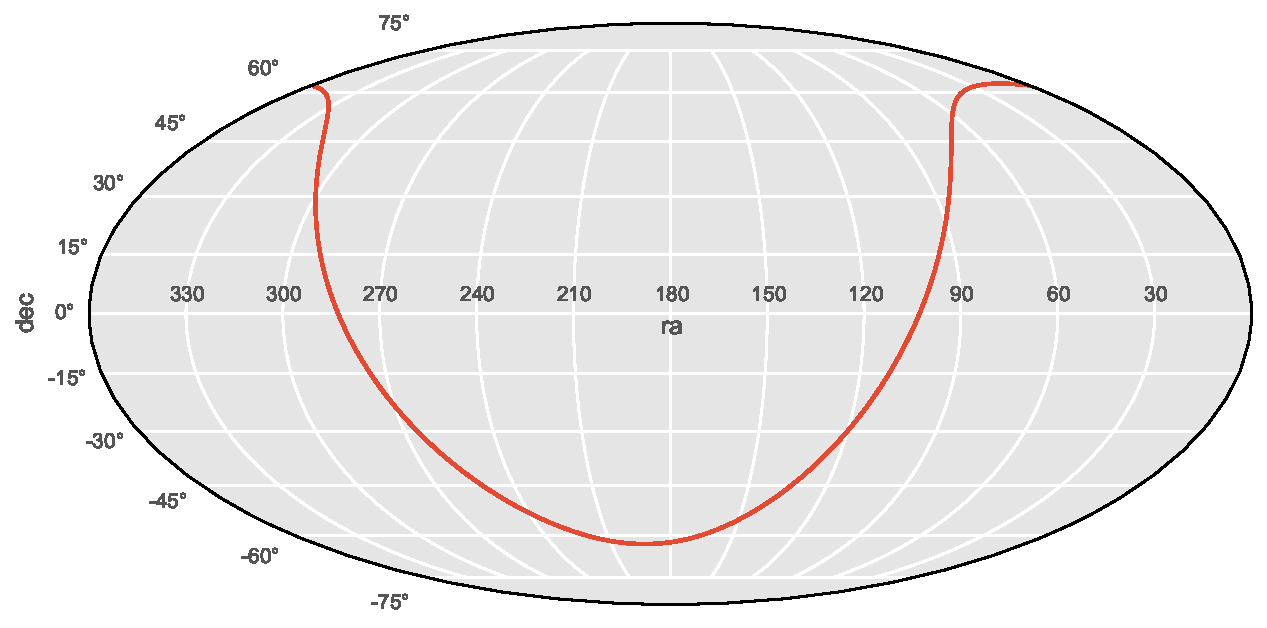
\includegraphics[width=\textwidth]{figures/map_mollweide}
	\caption[The Mollweide projection of the celestial sphere]{This is the Mollweide projection
		of the celestial sphere under the equatorial coordinate system. The red line indicates
		the plane of the Milky Way. Unless otherwise stated, all maps in the thesis use this
		configuration.To avoid cluttering, the coordinate labels will not be shown on later maps.}
	\label{fig:mollweide} \index{Mollweide projection}
\end{figure}

\section{SDSS Dataset}
\label{sec:datasets}
The main dataset in our investigation comes from the SDSS, a comprehensive survey of the
Northern Sky that began operation in 2000. This dataset consists of 800 million objects, covering
about a third of the sky \cite{alam15}. Figure \ref{fig:coverage} shows the coverage of the survey.
For each object, we are given 11 features:
	\begin{itemize}
		\item The PSF magnitude in each of the five ugriz bands.
		\item The Petrosian magnitude in each of the five ugriz bands.
		\item The Petrosian radius in the r-band.
	\end{itemize}
Only 2.8 million out of the 800 million objects have been spectroscopically classified into three
classes: galaxies, quasars, and stars. From Figure
\ref{fig:class_dist_sdss}, we can see that the majority of the labelled objects are galaxies. This leads to
a problem of class imbalance. In chapter
\ref{cha:ml}, we will discuss a few measures that can minimise any bias toward the
dominant class during classification. Another potential issue is that the classes
are not uniformly distributed across the sky, as shown in Figure \ref{fig:training_dist}.


\begin{figure}[tbp]
	\centering
	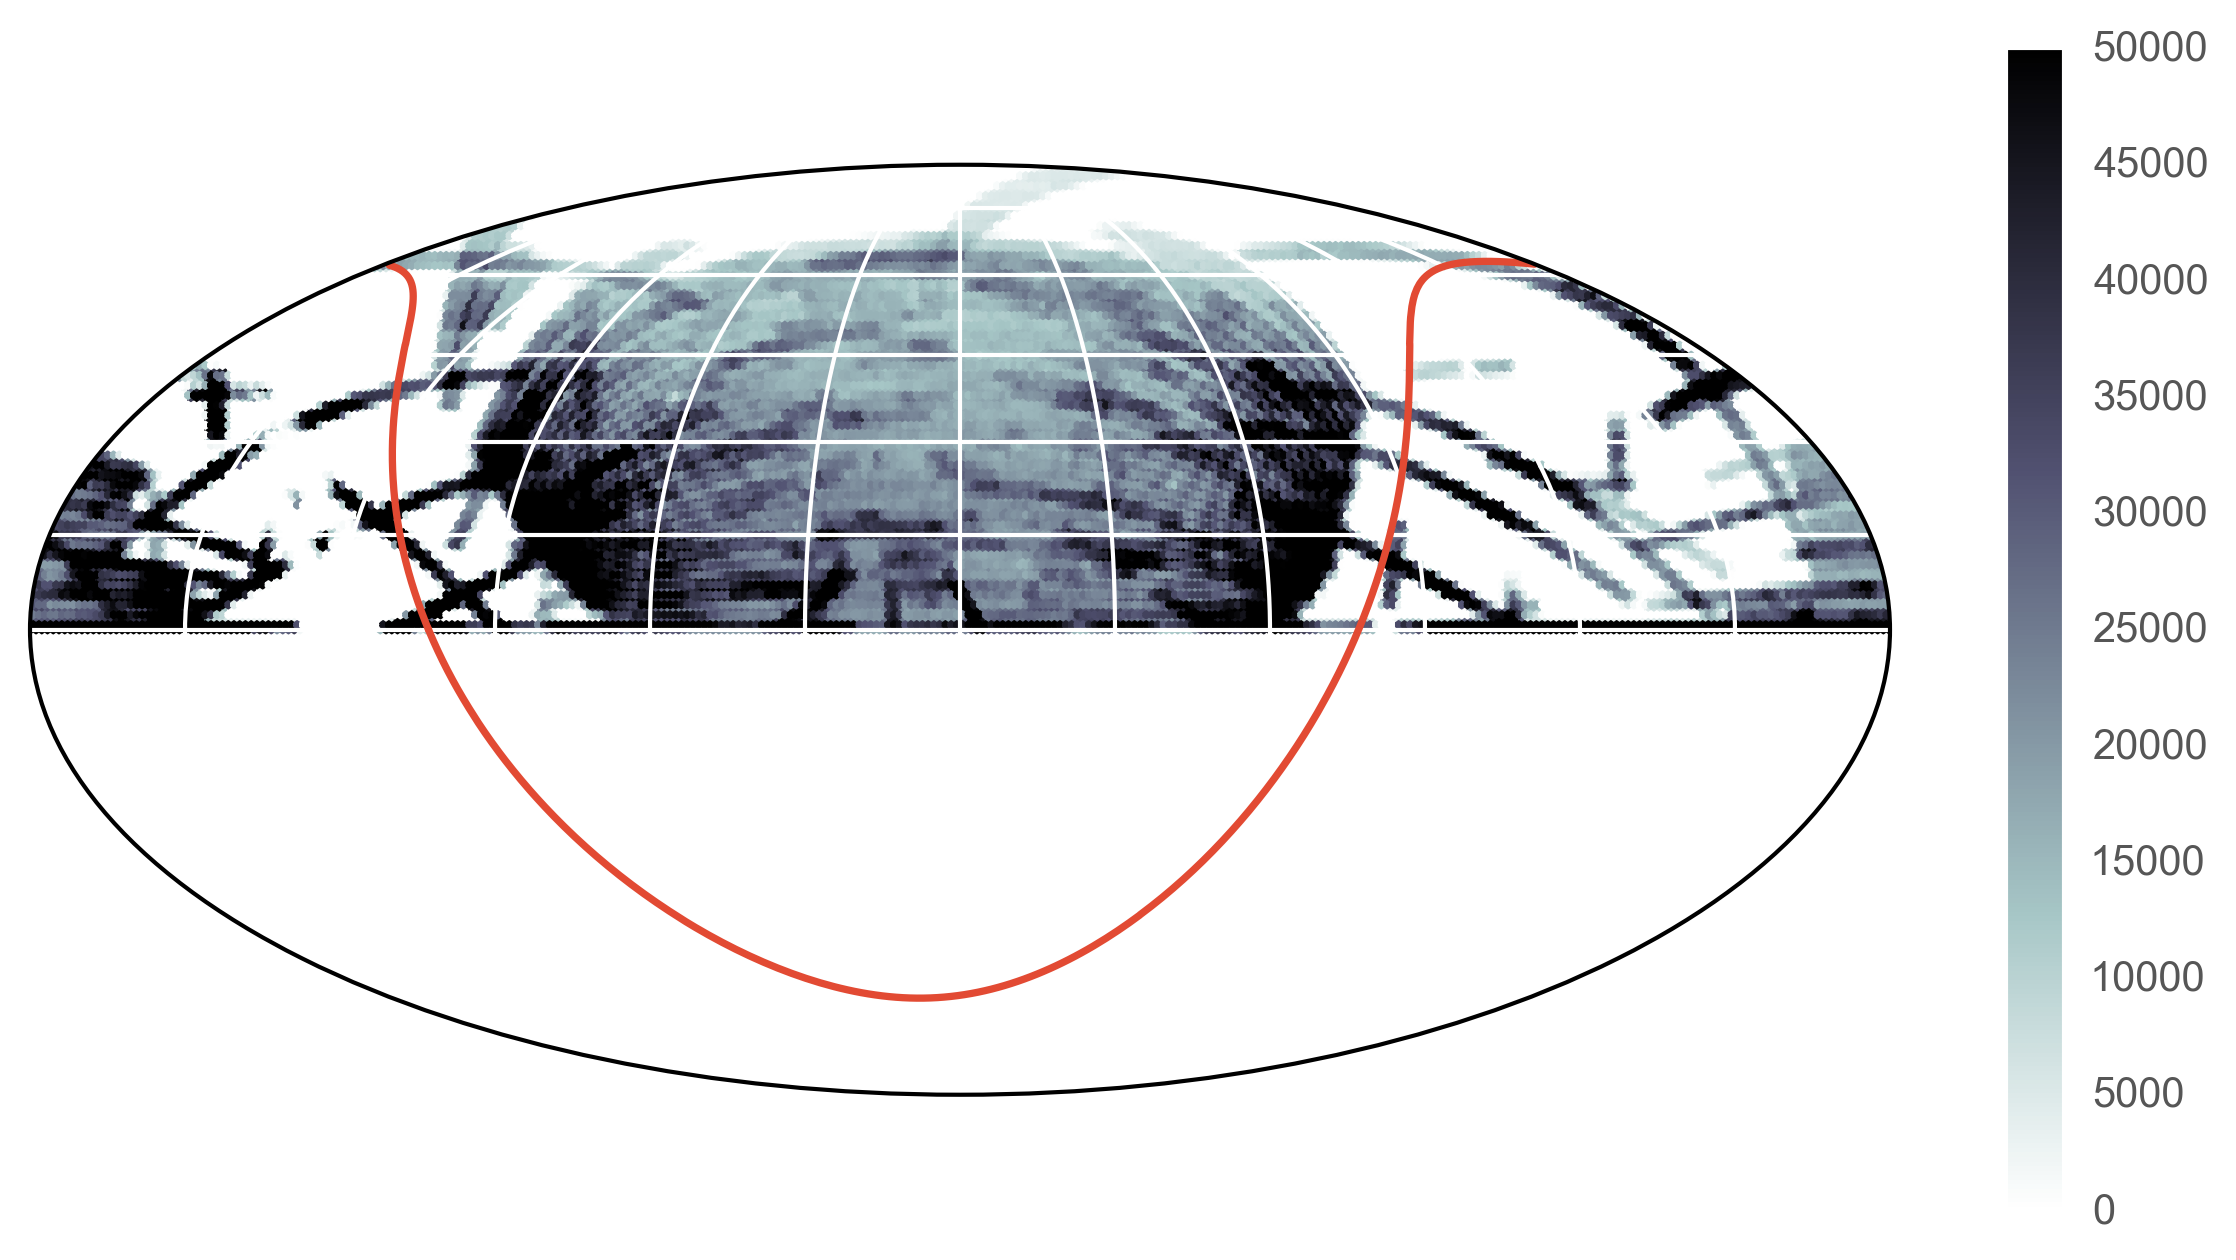
\includegraphics[width=\textwidth]{figures/map_prediction_forest_all}
	\caption[The coverage of the SDSS]{Since 2000, the SDSS has managed to cover one third
		of the celestial sphere. Here we show the
		distribution of the 800 million scanned objects in the survey.
		 Note that the coverage is not uniform. A darker colour
		corresponds to more objects being scanned in a particular area.}
	\label{fig:coverage}
\end{figure}

\begin{figure}[tbp]
	\centering
	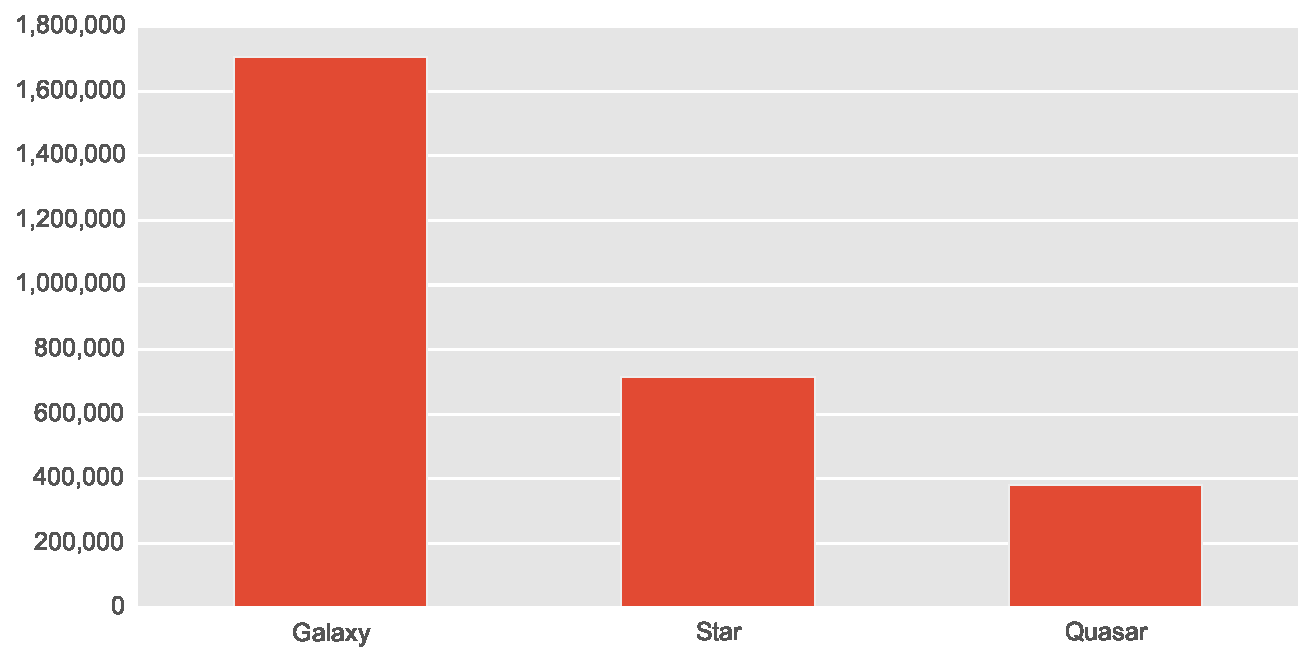
\includegraphics[width=\textwidth]{figures/bar_training_class_distribution}
	\caption[Histogram of the labelled objects in the SDSS]{Around 2.8 million
		objects in the SDSS has been spectroscopally classified into three classes: galaxies,
		stars, and quasars. This figure shows the histogram of the classes.
		Observe how we have four times as many galaxies as quasars.}
	\label{fig:class_dist_sdss}
\end{figure}

\begin{figure}[p]
	\centering
	\begin{subfigure}{\textwidth}
		\centering
		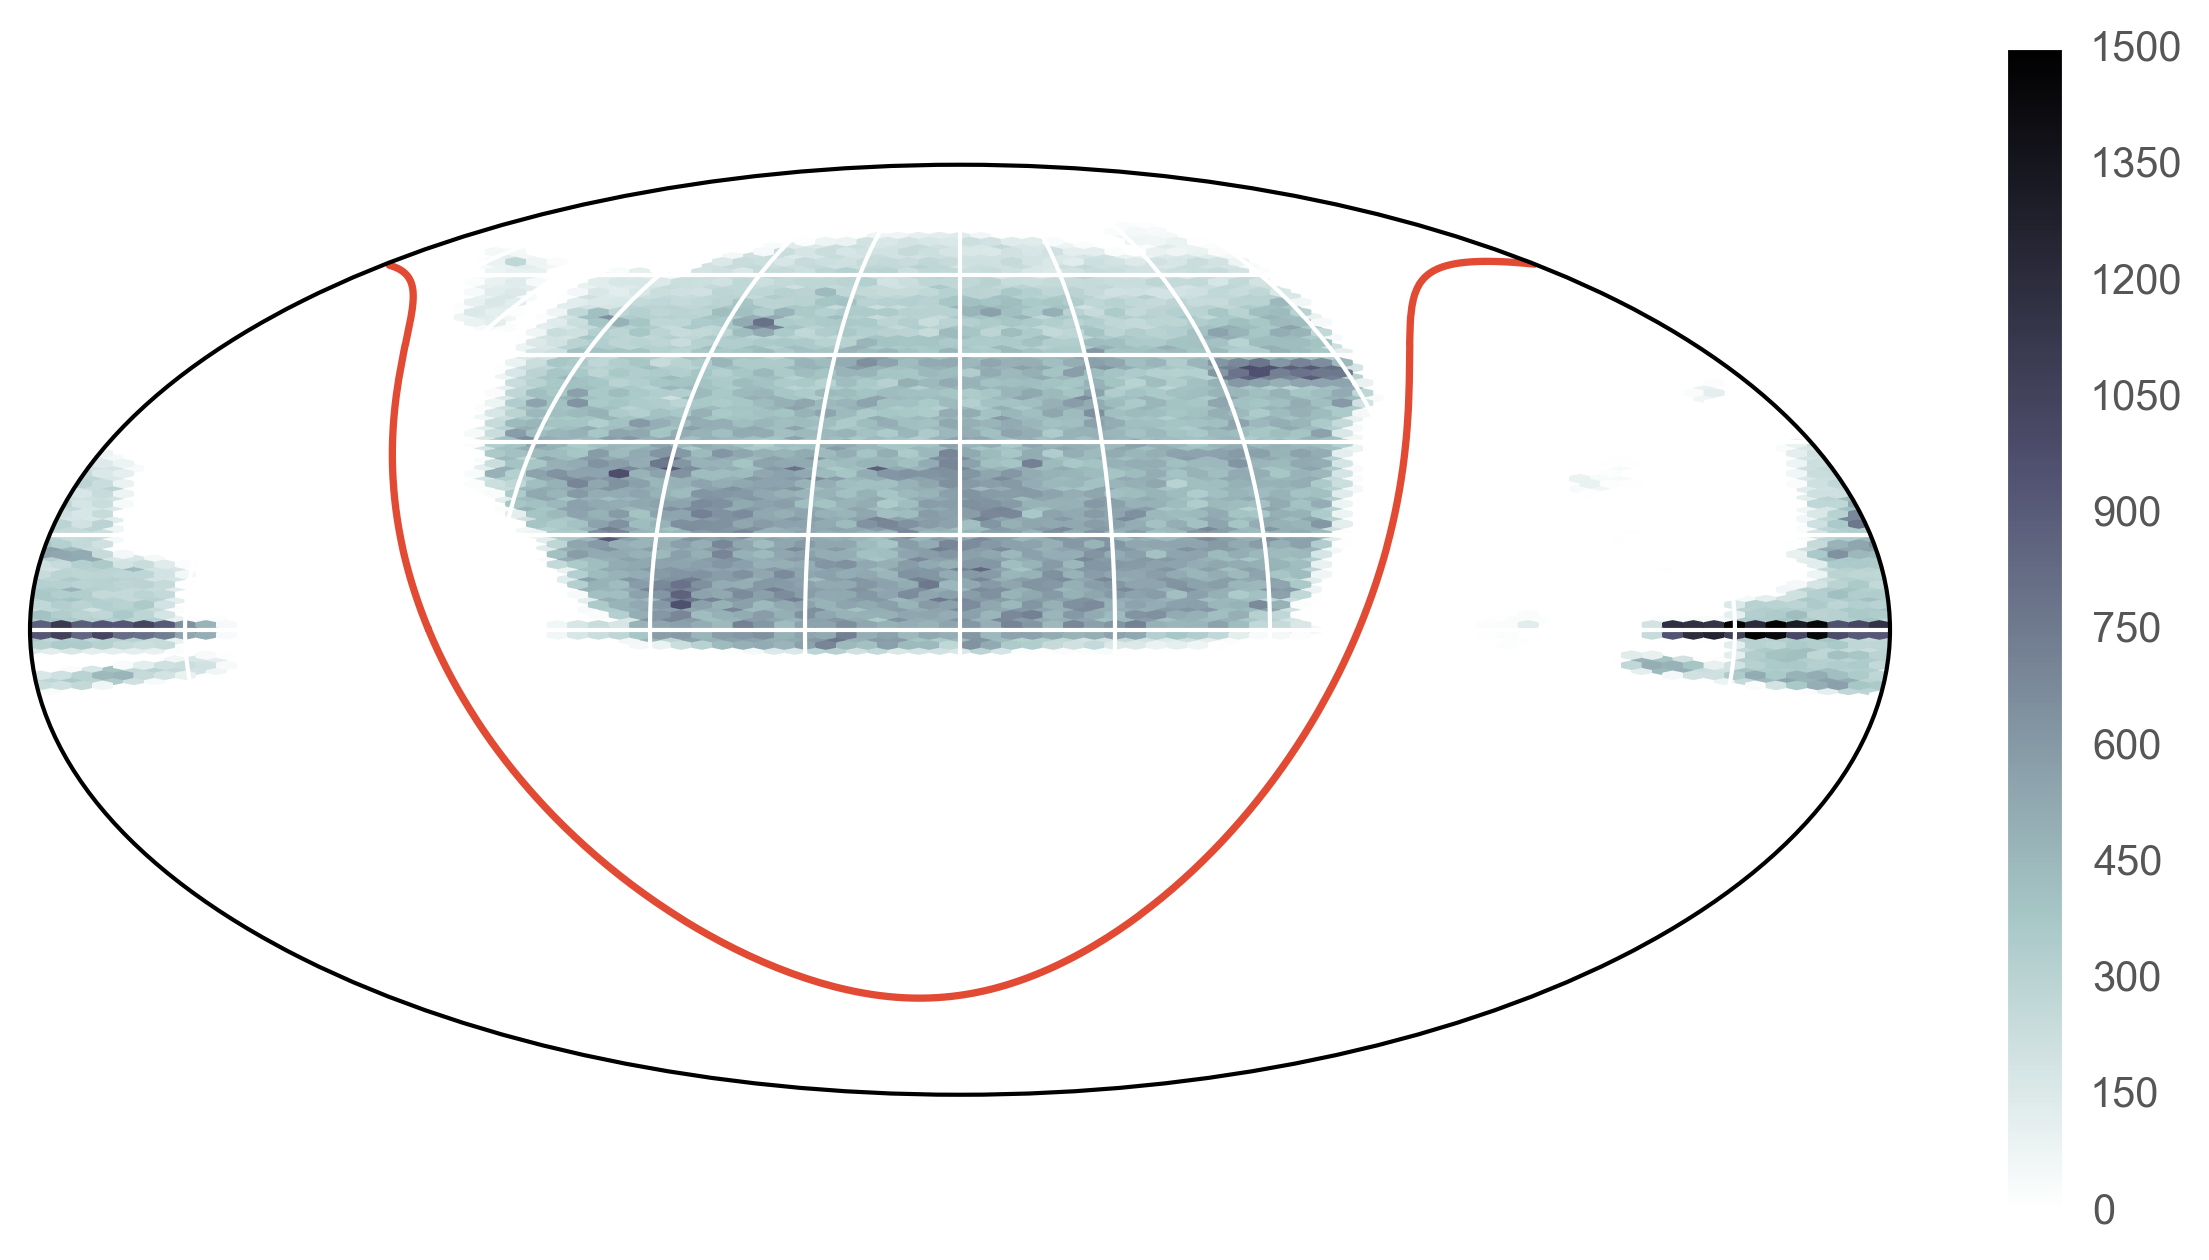
\includegraphics[width=0.73\textwidth]{figures/map_train_galaxies}
		\caption{The distribution of galaxies.}
		\label{fig:training_g}
	\end{subfigure}\\
	\begin{subfigure}{\textwidth}
		\centering
		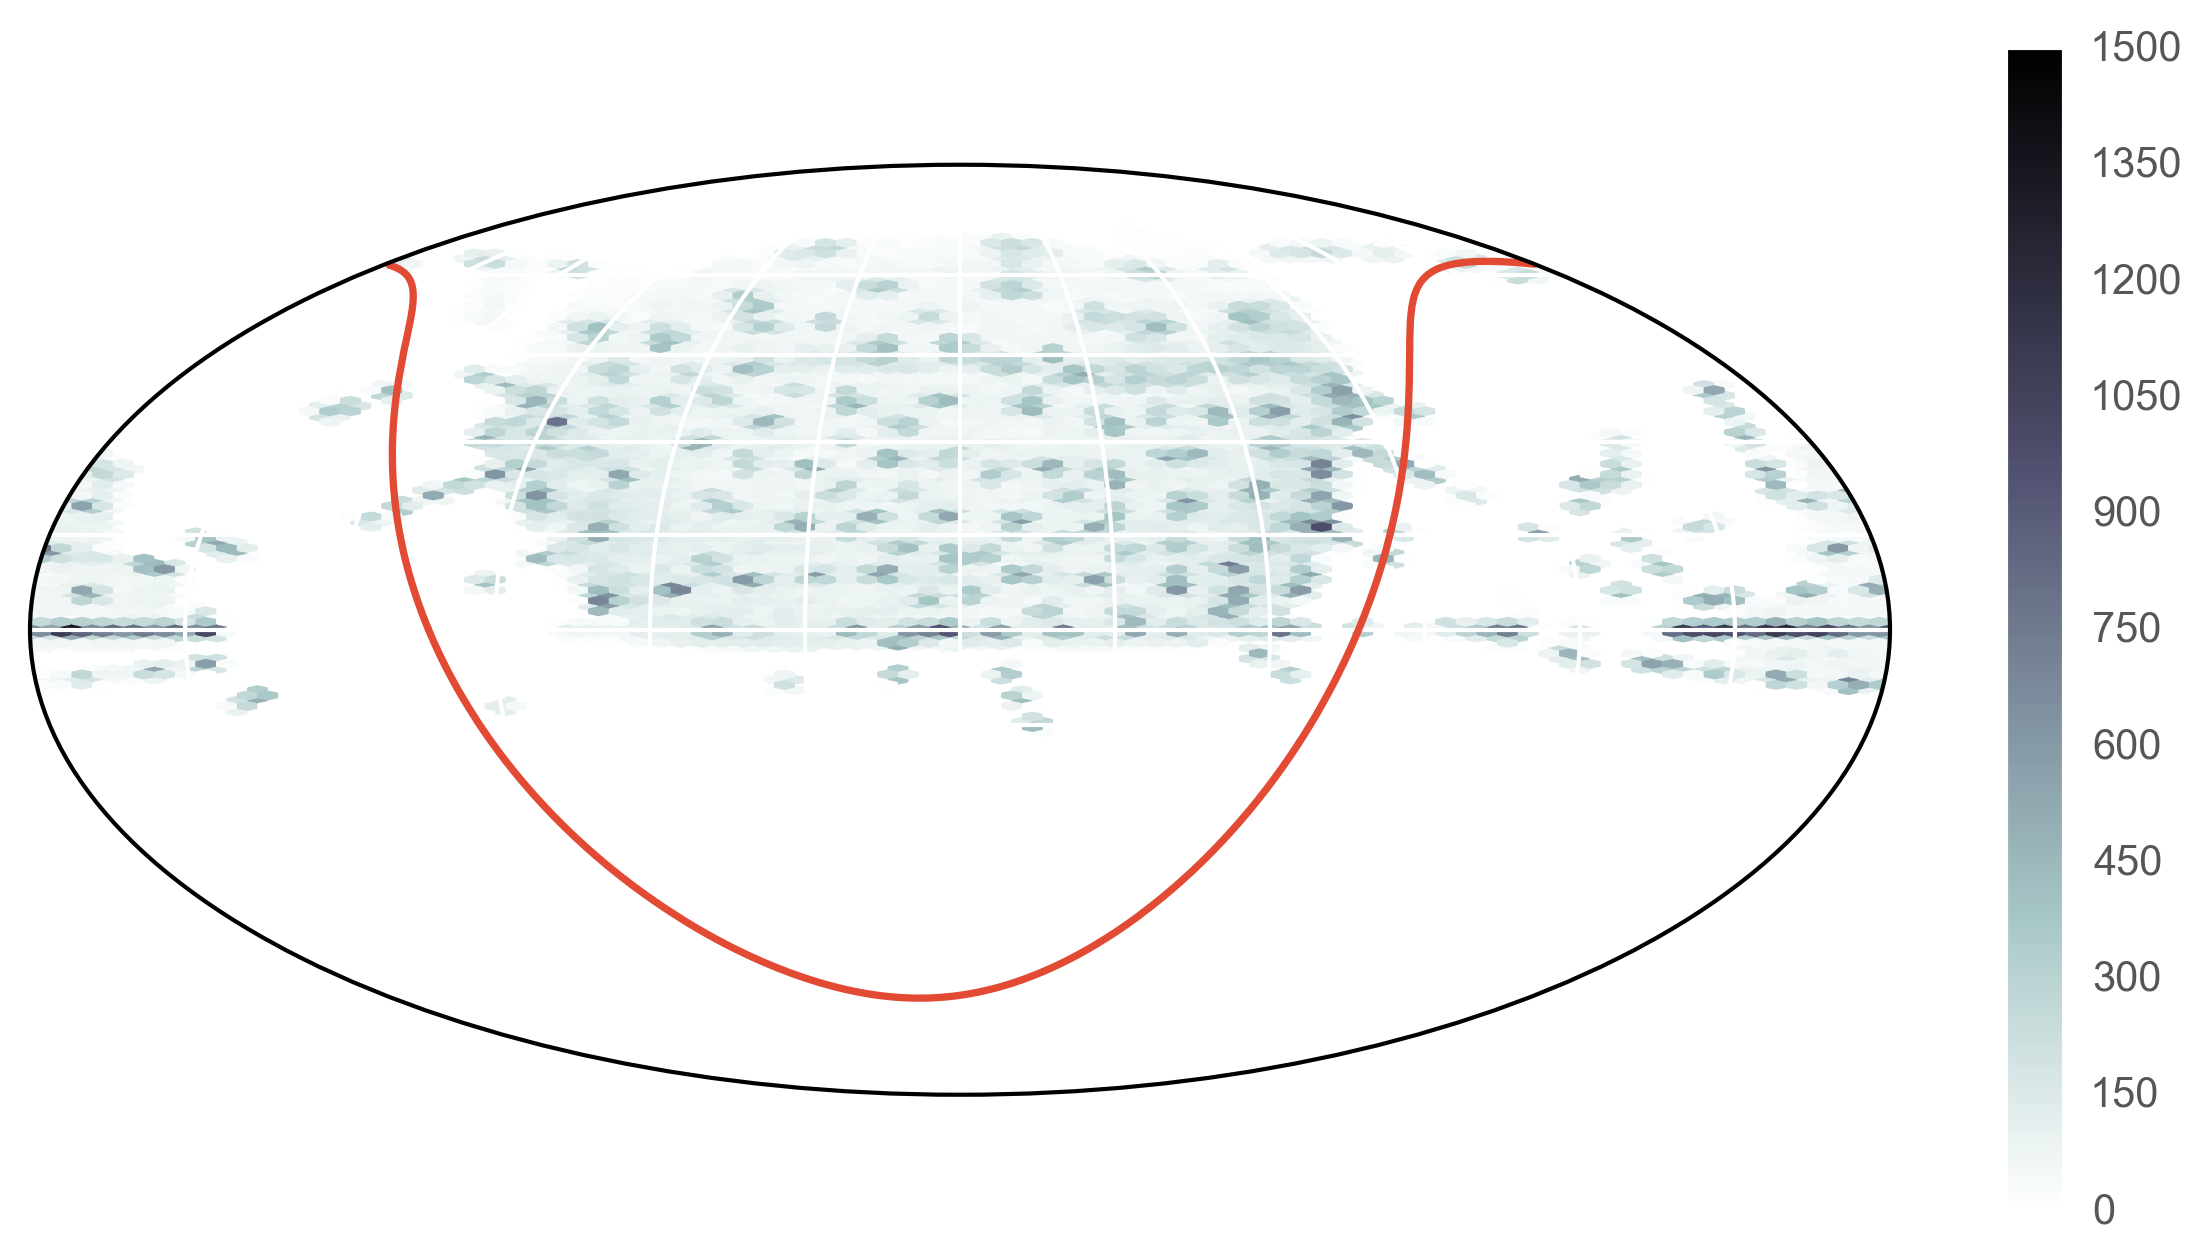
\includegraphics[width=0.73\linewidth]{figures/map_train_stars}
		\caption{The distribution of stars.}
		\label{fig:training_s}
	\end{subfigure}
	\begin{subfigure}{\textwidth}
		\centering
		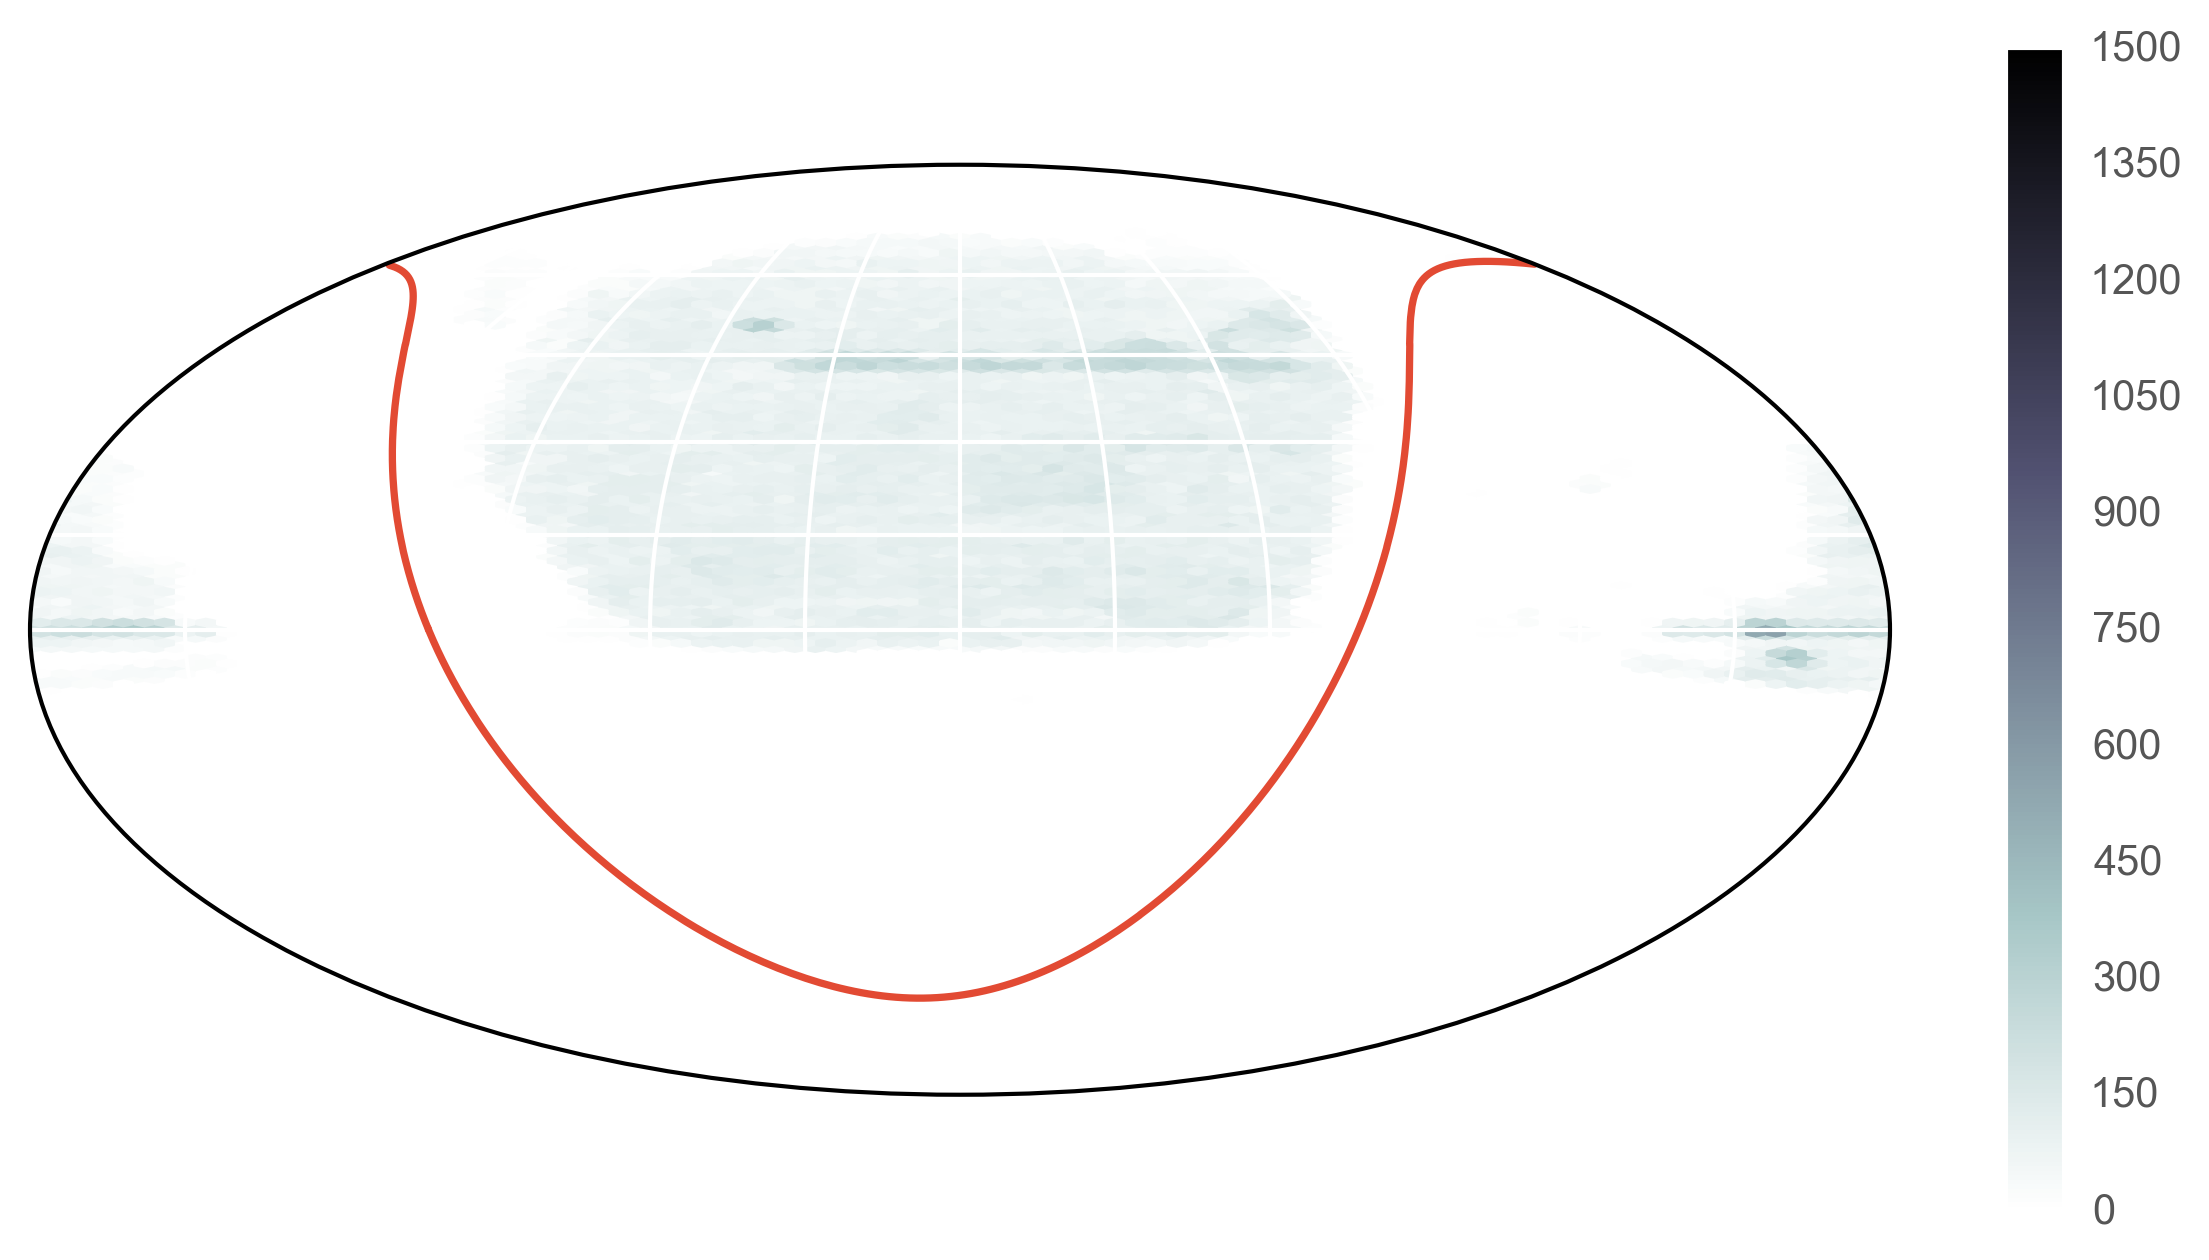
\includegraphics[width=0.73\linewidth]{figures/map_train_quasars}
		\caption{The distribution of quasars.}
		\label{fig:training_q}
	\end{subfigure}
	\caption[Distribution map of labelled objects in the SDSS]{The distribution map of
		the 2.8 million labelled objects in the SDSS: Observe that the
		galaxies are mostly uniformly distributed in the survey, while the stars are not.
		We also do not have a lot of examples of quasars.}
	\label{fig:training_dist}
\end{figure}

\begin{figure}[tbp]
	\centering
	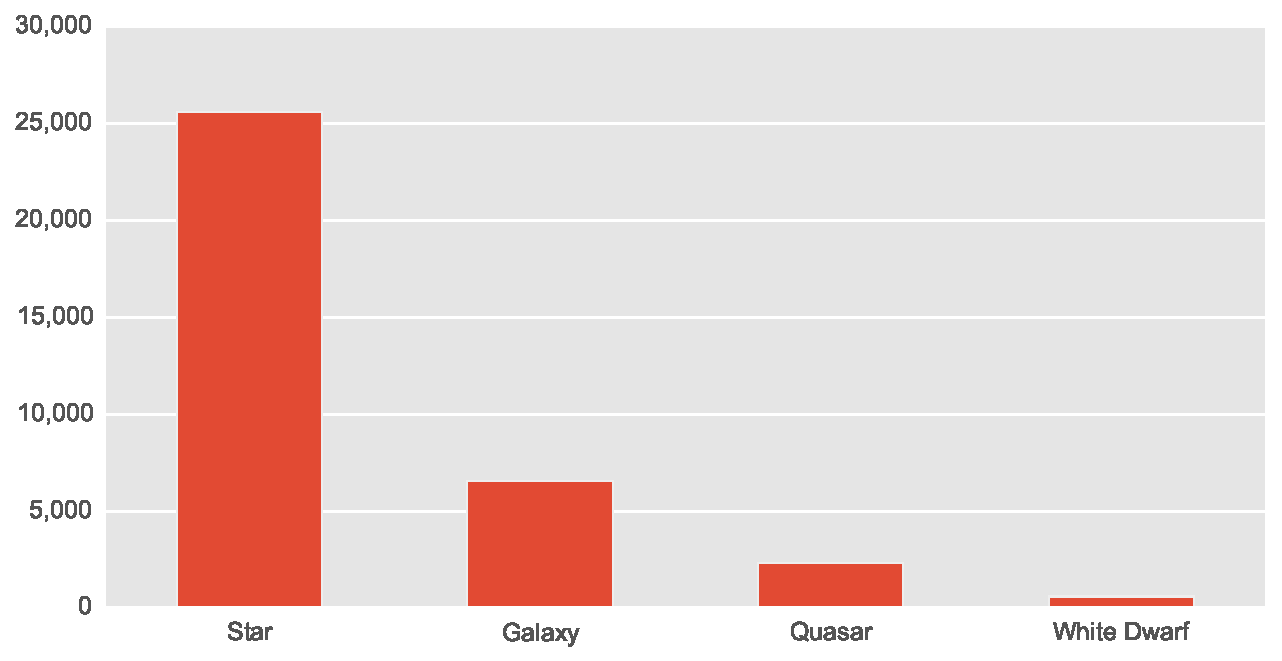
\includegraphics[width=\textwidth]{figures/bar_vstatlas_class_distribution}
	\caption[Histogram of the labelled objects in the VST-ATLAS]{In the VST-ATLAS dataset,
		we are provided with 35,000 objects classified into four classes: stars, galaxies,
		quasars, and white dwarfs. This figure shows the histogram of the classes.
		The class imbalance problem is still present is this dataset.}
	\label{fig:class_dist_vst}
\end{figure}

\section{VST-ATLAS Dataset}
A second and much smaller dataset comes from a more recent survey, the VST-ATLAS. This project
aims to survey 4500 deg$^2$ of the Southern Sky to roughly the same depth as the SDSS
\cite{shanks15}.
There are 35,000 objects in total which have been classified by an expert into four classes
this time: stars, galaxies, quasars, and white dwarfs. For each object, we are provided
with 5 features, a calibrated r-band magnitude and four colour indices.
As we can see from Figure \ref{fig:class_dist_vst}, the problem of class imbalance is even worse in this dataset. We 
have, for example, 25 times more stars than white dwarfs. Since research is still on-going, 
the coordinates of the objects are not yet publicly available.

For more information on how to obtain the datasets, refer to the Appendix.


\section{Dust Extinction}
To do: write about three sets of reddening corrections: \cite{schlegel98}, \cite{schlafly11},
and \cite{wolf14}.

\begin{figure}[tbp]
	\centering
	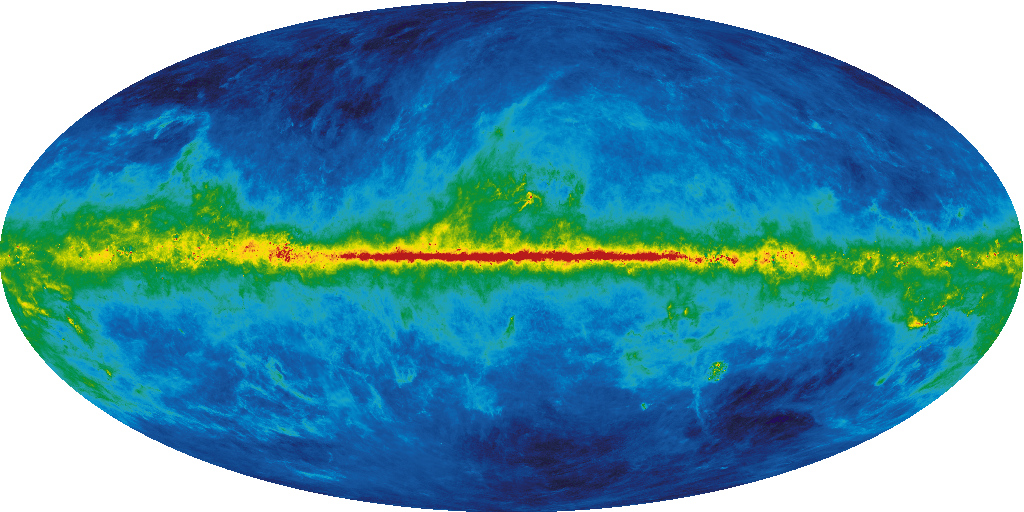
\includegraphics[width=\textwidth]{figures/galactic_reddening_ebv_map_sfd98}
	\caption[Galactic reddening map (SFD98)]{Galactic reddening map (SFD98). Source: LAMBDA}
	\label{fig:reddening}
\end{figure}


%%% Local Variables: 
%%% mode: latex
%%% TeX-master: "thesis"
%%% End: 
